%versi 2 (8-10-2016)
\chapter{Landasan Teori}
\label{chap:teori}

\section{Pengambilan Keputusan}
\subsection{Definisi Pengambilan Keputusan}
Pengambilan keputusan merupakan suatu proses intelektual dalam memilih suatu tindakan dari banyak alternative yang ada, untuk mendapatkan solusi dalam menyelesaikan suatu masalah. (dikutip dari journal decision making).

\subsection{Jenis Keputusan} 
Pengambilan keputusan dapat dibagi menjadi 3 jenis yaitu :  sumber(https://ejournal.bsi.ac.id/ejurnal/index.php/Bianglala/article/view/565).
\begin{itemize}
	\item Keputusan terstruktur
Keputusan terstruktur adalah keputusan yang bersifat rutin dan berulang sehingga dapat diprogram. Keputusan terstruktur sudah memiliki suatu prosedur atau syarat yang harus dipenuhi untuk menyelesaikan masalah tersebut. Keputusan ini  dilakukan pada manajemen tingkat bawah. Contoh dari keputusan ini adalah keputusan penagihan piutang.
	
	\item Keputusan semi terstruktur
Keputusan semi terstruktur adalah keputusan yang sebagian bersifat terstruktur dan sebagian lagi bersifat tidak terstruktur sehingga keputusan ini bersifat rumit dan membutuhkan perhitungan dan analisis yang terperinci. Keputusan ini dilakukan pada manajemen tingkat atas. Contoh dari keputusan ini adalah keputusan alokasi dana untuk promosi suatu produk. 

	\item Keputusan tidak terstuktur
Keputusan tidak terstruktur adalah keputusan yang bersifat tidak berulang dan tidak selalu terjadi, dimana tidak ada metode khusus untuk menyelesaikan masalah tersebut. Keputusan ini dilakukan pada manajemen tingkat atas. Contoh dari keputusan ini adalah keputusan untuk memilih rumah untuk dibeli.
\end{itemize}

\subsection{Tahap-tahap Pengambilan Keputusan}
Ada beberapa tahapan yang harus diperhatikan dalam pengambilan keputusan. Menurut Simon(1977) tahapan tersebut terdiri dari : (Decision and bi 9 edition)
\begin{enumerate}
	\item Tahap intelijen
Pada tahap ini seorang pembuat keputusan menelusuri dan memeriksa kenyataan dan berusaha untuk menentukan masalah, mengidentifikasi penyebab dan gejala masalah tersebut,menentukan seberapa besar dampak yang disebabkan, dan mengidentifikasi masalah tersebut.
	\item Tahap desain
Pada tahap ini masalah yang ada dianalisis dan dipahami serta mencari atau mengembangkan suatu tindakan yang mungkin untuk dijadikan suatu solusi. Pada tahap ini dibangun suatu model yang merepresentasikan suatu sistem. Model tersebut kemudian dites dan divalidasi. Proses pemodelan mengonseptualisasikan masalah dan memisahkannya ke dalam bentuk kuantitaif atau kualitatif.
	\item Tahap pemilihan
Pada tahap ini dibuat suatu keputusan yang nyata dan diambil suatu komitmen untuk mengikuti suatu tindakan tertentu. Tahap ini meliputi pencarian, evaluasi, dan rekomendasi dari solusi yang tepat untuk model.
	\item Tahap implementasi
Pada tahap ini, solusi yang direkomendasikan diimplementasikan ke dalam suatu permasalahan yang nyata.

\begin{figure}[H]
	\centering  
	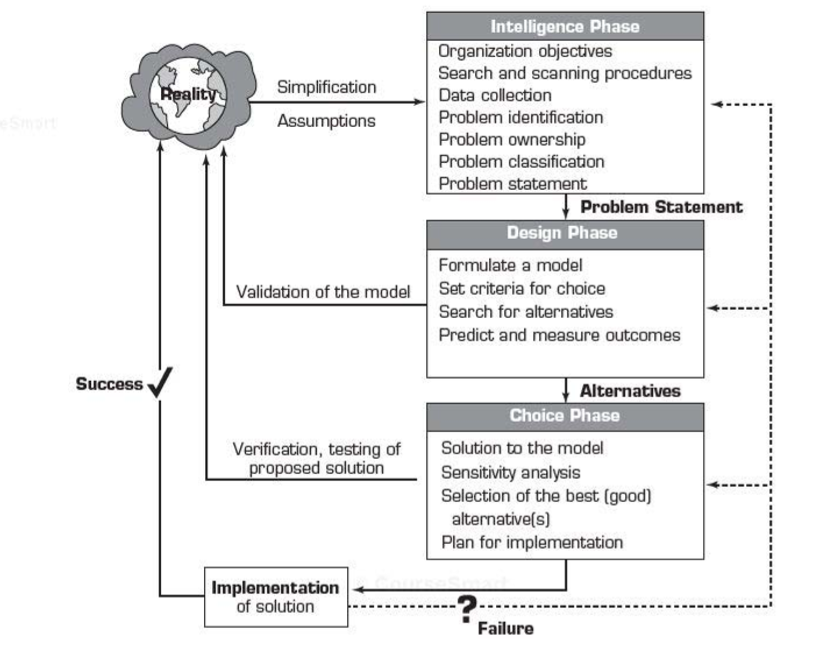
\includegraphics[scale=0.5]{tahapan_keputusan}  
	\caption[Tahap-tahap dalam pengambilan keputusan]{Tahap-tahap dalam pengambilan keputusan} 
	\label{fig:tahapan_keputusan} 
\end{figure} 

Gambar \ref{fig:tahapan_keputusan} menunjukan tahapan-tahapan yang harus dilalui untuk menyelesaikan masalah dan dari gambar tersebut terlihat bahwa kegagalan pada suatu tahap mengakibatkan seorang pembuat keputusan untuk mundur ke tahap sebelumnya.
	
\end{enumerate}

\section{Sistem Pendukung Keputusan}
\subsection{Definisi Sistem Pendukung Keputusan} 
Menurut Raymond McLeod (1998) Sistem Pendukung Keputusan adalah sistem penghasil informasi spesifik yang bertujuan untuk memecahkan suatu masalah tertentu yang dilakukan oleh manager pada berbagai tingkatan. 

Menurut Litle(1970) Sistem Pendukung Keputusan adalah suatu sistem informasi berbasis komputer yang dapat menghasilkan berbagai alternatif keputusan dan berfungsi untuk membantu manajemen dalam menangani berbagai masalah yang bersifat terstruktur ataupun tidak terstruktur dengan menggunakan data dan model.

Secara umum Sistem Pendukung keputusan adalah sebuah sistem yang mampu memberikan kemampuan, baik kemampuan pemecahan masalah maupun kemampuan pengkomunikasian untuk masalah semi terstruktur.

Sumber(https://ejournal.bsi.ac.id/ejurnal/index.php/Bianglala/article/view/565)

\subsection{Komponen Sistem Pendukung Keputusan}

Sistem Pendukung keputusan terdiri dari beberapa komponen,yaitu :
\begin{enumerate}
	\item Subsistem Manajemen Data
Subsistem manajemen data menyediakan basis data yang didalamnya mengandung data yang relevan dan dikelola oleh perangkat lunak yang disebut \textit{Database Management System} (DBMS).
	\item Subsistem Manajemen Model
Subsistem Manajemen Model berfungsi sebagai pengelola model keuangan, statistik, ilmu manajemen, atau model kuantitatif lainnya yang menyediakan kemampuan analitik dan manajemen perangkat lunak yang tepat. Perangkat lunak ini disebut \textit{model base management system} (MBMS).
	\item Subsistem Antarmuka Pengguna
Subsistem antarmuka pengguna berfungsi sebagai komponen yang digunakan pengguna untuk berinteraksi dan memberi perintah terhadap sistem pendukung keputusan. 
	\item Subsistem manajemen Berbasis Pengetahuan
Subsistem manajemen berbasis pengetahuan dapat berfungsi sebagai pendukung untuk subsistem lain atau bertindak sebagai komponen yang independen. Subsistem ini memberikan intelegensi untuk memperluas pengetahuan seorang pengambil keputusan.

\begin{figure}[H]
	\centering  
	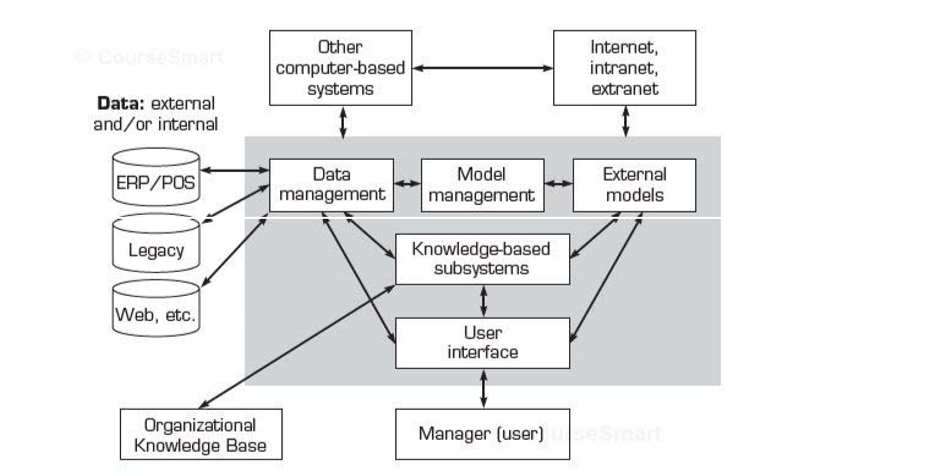
\includegraphics[scale=0.5]{komponen}  
	\caption[Skematik SPK]{Skematik SPK} 
	\label{fig:komponen} 
\end{figure}

\end{enumerate}
	
\section{Metode Brown Gibson}
Metode Brown Gibson adalah pemodelan matematika yang digunakan untuk mendukung pengambilan keputusan, dimana keputusan tersebut mempertimbangkan faktor objektif yang dikombinasikan dengan pertimbangan subjektif. Metode Brown Gibson menggunakan \textit{preference theory} dan aritmatika sederhana.
Langkah-langkah penerapan Metode Brown Gibson :
\begin{enumerate}
	\item Menetapkan alternatif solusi yang ada
	\item Menetapkan kriteria-kriteria yang menjadi pertimbangan. Kriteria tersebut dapat dikelompokkan mejadi 2 jenis, yaitu faktor objektif dan faktor subjektif. Faktor subjektif merupakan kriteria yang nilainya bersifat kualitatif atau tidak mempunyai nilai numerik, dan faktor objektif yang nilainya bersifat kuantitatif atau mempunyai nilai numerik.
	\item Menetapkan \textit{preference of measurment} dari faktor objektif yang ada.	
	\item Menghitung nilai \textit{Objective faktor weight} (OFW) dengan menentukan nilai performasi setiap faktor objektif yang ada dengan rumus 
\begin{figure}[H]
	\centering  
	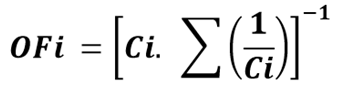
\includegraphics[scale=0.5]{ofi}   
\end{figure}

Dimana $\Sigma OFi=1$
\item Menghitung \textit{Subjective faktor weight} (SFW)dengan melakukan \textit{pairwaise comparison} antar faktor subjektif yang ada, dengan pemberian bobot sebagai berikut : 
\begin{itemize}
	\item Lebih baik diberi point = 1
	\item Sama baik diberi point masing-masing = 1 
	\item Sama jelek diberi point masing-masing = 0
	\item lebih jelek diberi point = 0
\end{itemize}
\item Menghiutng \textit{Objective factor decision weight} (OFDW) untuk setiap faktor objektif yang ada terhadap alternatif pilihan yang tersedia.
\item Menghitung \textit{Subjective factor decision weight} (SFDW) untuk setiap faktor subjektif yang ada terhadap alternatif pilihan yang tersedia.
\item Menghitung \textit{Subjective factor meassure} (SFM) untuk setiap faktor subjektif yang ada terhadap alternatif pilihan yang tersedia dengan rumus :
$SFMc = SFWc * SFDWc$
\item Menghitung Decision Weight setiap alternatif pilihan untuk setiap faktor Objektif yang ada dengan rumus :

$\mbox{Decision Weight} \mbox{{\tiny (Choice c)}} = \Sigma( \mbox{OFW} \mbox{{\tiny(Factor f)}} * \mbox{OFDW} \mbox{{\tiny (Choice c,factor f)}})+(1-\mbox{OFW} \mbox{{\tiny (Factor F)}}*\mbox{SFM} \mbox{{\tiny (Choice c)}}$

\item Jumlahkan semua \textit{Decision weight } dari setiap faktor objektif yang ada untuk semua pilihan alternatif yang ada. Alternatif pilihan dengan total nilai tertinggi merupakan pilihan rumah yang paling optimal. 
	
\end{enumerate}

\section{Rumah}
Rumah adalah salah satu kebutuhan pokok manusia yang berfungsi sebagai tempat berlindung dan beristirahat. Rumah menurut UU No.4 Tahun 1992 tentang perumahan dan pemukiman adalah bangunan yang berfungsi sebagai tempat tinggal atau hunian dan sarana pembinaan keluarga.

\subsection{Fungsi Rumah}
Menurut A.Turner (dalam jenie, 2001:45 ), rumah memiliki tiga fungsi utama, yaitu :
\begin{enumerate}
	\item Rumah sebagai identitas keluarga,hal ini diwujudkan melalui kualitas suatu hunian untuk melindungi  penghuni dari iklim setempat.
	\item Rumah sebagai penunjang kesempatan keluarga untuk berkembang dalam kehidupan sosial budaya dan ekonomi atau fungsi pengemban keluarga.
	\item Rumah sebagai penunjang rasa aman, rumah sebagai penunjang rasa aman memiliki arti adanya jaminan rasa aman dimasa depan setelah mendapatkan rumah, yang diwujudkan melalui jaminan keamanan atas lingkungan dan jaminan kepemilikan rumah dan lahan. 
\end{enumerate}
\subsection{Jenis Rumah}
Terdapat 8 jenis perumahan yang dikemukakan oleh Richard Untermann dan Robert Small(1986) dalam buku Perancangan Tapak untuk Perumahan, diantaranya :
\begin{enumerate}
	\item Rumah Tinggal Tunggal \\
Rumah tinggal tunggal adalah rumah tinggal yang berdiri sendiri dan biasanya digunakan oleh satu keluarga. Rumah tinggal tunggal dibangun di atas tanah yang luas sehingga rumah tersebut dikeliling halaman dan juga jarak antara satu rumah dengan rumah yang lainnya berjauhan.
	\item Rumah Tinggal Koppel \\
Rumah tinggal koppel adalah rumah yang disekat sama besar antara sisi kiri dan kanannya.Biasanya rumah tinggal koppel ini untuk disewakan.
	\item Rumah Gandeng \\
Rumah gandeng adalah rumah yang berasal dari rumah tradisional berlantai dua, yang terletak di atas sebidang tanah yang sempit. Fungsi-fungsi dasar rumah ini terletak di lantai bawah.
	\item Rumah Kota \\
Rumah kota sama seperti rumah gandeng dengan penambahan tempat parkir di dalam bangunannya. Rumah kota nyaman ditempati untuk sebuah keluarga tunggal.
	\item Rumah Susun \\
Rumah susun adalah rumah yang mampu menyesuaikan berbagai konfigurasi. Rumah susun umumnya mempunyai ruang-ruang yang berada di luar unit-unit rumah tersebut.
	\item Rumah berpekarangan Dalam \\
Rumah berpekarangan dalam adalah variasi dari rumah 'ranch' berlantai satu tradisional, dengan pintu masuk di bagian tengah, ruang tamu terletak di sisi dan ruang tidur terletak pada sisi lainnya.
	\item Maisonet
Rumah maisonet adalah rumah berkapasitas tinggi dan bertingkat rendah. Rumah ini terdiri dari dua lantai umumnya lantai satu untuk kegiatan umum dan lantai dua khusus untuk ruang tidur.
	\item Rumah teras bertingkat \\
Rumah gandeng dan berpekarangan dalam dapat dibuat menjenjang ke atas maupun ke bawah sebuah perbukitan untuk meningkatkan arah pandangan, dan memberikan orientasi yang lebih baik dan juga memungkinkan taman atau teras berada di atas atap dari unit dibawahnya.
	
\end{enumerate}
































\section{Skripsi}
\label{sec:skripsi} 
 
Rencananya akan diisi dengan penjelasan umum mengenai buku skripsi.

\dtext{11-12} 

\section{\LaTeX}
\label{sec:latex}

Mengapa menggunakan \LaTeX{} untuk buku skripsi dan apa keunggulan/kerugiannya bagi mahasiswa dan pembuat template. 

\dtext{13-14}


\section{Template Skripsi FTIS UNPAR}
\label{sec:template}
 
Akan dipaparkan bagaimana menggunakan template ini, termasuk petunjuk singkat membuat referensi, gambar dan tabel.
Juga hal-hal lain yang belum terpikir sampai saat ini. 
 
\dtext{15-16}

\subsection{Tabel}  
Berikut adalah contoh pembuatan tabel. 
Penempatan tabel dan gambar secara umum diatur secara otomatis oleh \LaTeX{}, perhatikan contoh di file bab2.tex untuk melihat bagaimana cara memaksa tabel ditempatkan sesuai keinginan kita.

Perhatikan bawa berbeda dengan penempatan judul gambar gambar, keterangan tabel harus diletakkan di atas tabel!!
Lihat Tabel~\ref{tab:contoh1} berikut ini:

\begin{table}[H] %atau h saja untuk "kira kira di sini"
	\centering 
	\caption{Tabel contoh}
	\label{tab:contoh1}
	\begin{tabular}{cccc}
		\toprule
		& $v_{start}$ & $\mathcal{S}_{1}$ & $v_{end}$\\

		\midrule
		$\tau_{1}$ & 1 & 12& 20\\
		$\tau_{2}$ & 1 &  & 20\\
		$\tau_{3}$ & 1 & 9 & 20\\
		$\tau_{4}$ & 1 &  & 20\\

		\bottomrule
		
	\end{tabular} 
\end{table}
Tabel~\ref{tab:cthwarna1} dan Tabel~\ref{tab:cthwarna2} berikut ini adalah tabel dengan sel yang berwarna dan ada dua tabel yang bersebelahan. 
\begin{table}[H]
	\begin{minipage}[c]{0.49\linewidth}
		\centering
		\caption{Tabel bewarna(1)}
		\label{tab:cthwarna1}
		\begin{tabular}{ccccc}
			\toprule
			 & $v_{start}$ & $\mathcal{S}_{2}$ & $\mathcal{S}_{1}$ & $v_{end}$\\
			
			\midrule
			$\tau_{1}$ & 1 & 5 \cellcolor{green}& 12& 20\\
			$\tau_{2}$ & 1 & 8 \cellcolor{green}& & 20\\
			$\tau_{3}$ & 1 & 2/8/17 \cellcolor{green}& 9 & 20\\
			$\tau_{4}$ & 1 & \cellcolor{red}& & 20\\
			
			\bottomrule

		\end{tabular}
	\end{minipage}
	\begin{minipage}[c]{0.49\linewidth}
		
		\centering 
		\caption{Tabel bewarna(2)}
		\label{tab:cthwarna2}
		\begin{tabular}{ccccc}
			\toprule
			 & $v_{start}$ & $\mathcal{S}_{1}$ & $\mathcal{S}_{2}$ & $v_{end}$\\
			
			\midrule
			$\tau_{1}$ & 1 & 12& 5 \cellcolor{red} &20\\
			$\tau_{2}$ & 1 &  &  8 \cellcolor{green} &20\\
			$\tau_{3}$ & 1 & 9 & 2/8/17 \cellcolor{green} &20\\
			$\tau_{4}$ & 1 &   & \cellcolor{red} &20\\
			
			\bottomrule
		
		\end{tabular}
	\end{minipage}
\end{table}

 
\subsection{Kutipan}
\label{subs:kutipan} 
Berikut contoh kutipan dari berbagai sumber, untuk keterangan lebih lengkap, silahkan membaca file referensi.bib yang disediakan juga di template ini.
Contoh kutipan:
\begin{itemize}
	\item Buku:~\cite{berg:08:compgeom} 
	\item Bab dalam buku:~\cite{kreveld:04:GIS}
	\item Artikel dari Jurnal:~\cite{buchin:13:median}
	\item Artikel dari prosiding seminar/konferensi:~\cite{kreveld:11:median}
	\item Skripsi/Thesis/Disertasi:~\cite{lionov:02:animasi}~\cite{wiratma:10:following}~\cite{wiratma:22:later}
	\item Technical/Scientific Report:~\cite{kreveld:07:watertight}
	\item RFC (Request For Comments):~\cite{RFC1654}
	\item Technical Documentation/Technical Manual:~\cite{Z.500}~\cite{unicode:16:stdv9}~\cite{google:16:and7}
	\item Paten:~\cite{webb:12:comm}
	\item Tidak dipublikasikan:~\cite{wiratma:09:median}~\cite{lionov:11:cpoly}
	\item Laman web:~\cite{erickson:03:cgmodel}  
	\item Lain-lain:~\cite{agung:12:tango}
\end{itemize}    
  
\subsection{Gambar}

Pada hampir semua editor, penempatan gambar di dalam dokumen \LaTeX{} tidak dapat dilakukan melalui proses {\it drag and drop}.
Perhatikan contoh pada file bab2.tex untuk melihat bagaimana cara menempatkan gambar.
Beberapa hal yang harus diperhatikan pada saat menempatkan gambar:
\begin{itemize}
	\item Setiap gambar {\bf harus} diacu di dalam teks (gunakan {\it field} {\sc label})
	\item {\it Field} {\sc caption} digunakan untuk teks pengantar pada gambar. Terdapat dua bagian yaitu yang ada di antara tanda $[$ dan $]$ dan yang ada di antara tanda $\{$ dan $\}$. Yang pertama akan muncul di Daftar Gambar, sedangkan yang kedua akan muncul di teks pengantar gambar. Untuk skripsi ini, samakan isi keduanya.
	\item Jenis file yang dapat digunakan sebagai gambar cukup banyak, tetapi yang paling populer adalah tipe {\sc png} (lihat Gambar~\ref{fig:ularpng}), tipe {\sc jpg} (Gambar~\ref{fig:ularjpg}) dan tipe {\sc pdf} (Gambar~\ref{fig:ularpdf})
	\item Besarnya gambar dapat diatur dengan {\it field} {\sc scale}.
	\item Penempatan gambar diatur menggunakan {\it placement specifier} (di antara tanda  $[$ dan $]$ setelah deklarasi gambar.
	Yang umum digunakan adalah {\bf H} untuk menempatkan gambar {\bf sesuai} penempatannya di file .tex atau  {\bf h} yang berarti "kira-kira" di sini. \\
	Jika tidak menggunakan {\it placement specifier}, \LaTeX{} akan menempatkan gambar secara otomatis untuk menghindari bagian kosong pada dokumen anda.
	Walaupun cara ini sangat mudah, hindarkan terjadinya penempatan dua gambar secara berurutan. 	
	\begin{itemize}
		\item Gambar~\ref{fig:ularpng} ditempatkan di bagian atas halaman, walaupun penempatannya dilakukan setelah penulisan 3 paragraf setelah penjelasan ini.
		\item Gambar~\ref{fig:ularjpg} dengan skala 0.5 ditempatkan di antara dua buah paragraf. Perhatikan penulisannya di dalam file bab2.tex!
		\item Gambar~\ref{fig:ularpdf} ditempatkan menggunakan {\it specifier} {\bf h}.
	\end{itemize}
\end{itemize}
 
\dtext{17-18}
\begin{figure} 
	\centering  
	\includegraphics[scale=1]{ular-png}  
	\caption[Gambar {\it Serpentes} dalam format png]{Gambar {\it Serpentes} dalam format png} 
	\label{fig:ularpng} 
\end{figure} 

\dtext{19-20}
\begin{figure}[H]
	\centering  
	\includegraphics[scale=0.5]{ular-jpg}  
	\caption[Ular kecil]{Ular kecil} 
	\label{fig:ularjpg} 
\end{figure} 
\dtext{21-22}

\begin{figure}[ht] 
	\centering  
	\includegraphics[scale=1]{ular-pdf}  
	\caption[ {\it Serpentes} betina]{ {\it Serpentes} jantan} 
	\label{fig:ularpdf} 
\end{figure} 
 
 
